\chapter{The cost of errors} 

\label{Chapter 6}

\lhead{Chapter 6. \emph{The cost of errors}}
\vspace{3cm}
\newpage

% New Sections for Ami to read
% - Introduction that joins from past chapter: highlighted red. 

\noindent
The method, results and discussion of this Chapter appear in the submitted manuscript `The cost of errors: confusion analysis and the mental representation of familiar and unfamiliar digits' \cite{garrettWheel1}. The following Chapter can be thought of as the beginning of our second research stream that will examine the confusion of numbers.

\color{\Red}
\section{Chapter overview}
% Tie into Thesis overview
In Chapters 3 and 4, we assessed the properties of a cognitive system that judged whether a quantity was less than some critical value. As opposed to this somewhat coarse assessment of quantity, we often need to communicate the precise value of an item-set. As shown in Chapter 2, even our best self-reported estimates of quantity are usually under or over estimate set-size. For this reason, the precise evaluation of an item-set is usually accomplished through the process of counting.

Counting is a slow, accumulative and precise process of enumeration. The precision of counting has led many civilizations to develop non-symbolic numerals. Non-symbolic numerals, such as tallies and dice, are both a physical and symbolic representation of quantity. They communicate quantity through the sum of their items, and the canonical patterns those items form. For example, five sheep may be represented by the canonical tally of one diagonal and four vertical strokes. Although non-symbolic numerals are effective at communicating small quantities, they become error prone at larger counts (e.g., a tally of 500 sheep). In response, many cultures have also developed symbolic numeral systems.

Symbolic numerals map increments in quantity onto unique symbolic representations, for example, the Arabic digits 0--9. This allows the clear and precise communication of large item-sets. Humanity's progression in mathematics, science and trade has hinged upon the use of symbolic numerals, and necessitated a transition away from their non-symbolic counterparts. Today, symbolic numerals are used for trade, programming, security, cooking, and a host of other activities. The ubiquity of their use has made symbolic numerals inherent of the quantities they represent. Yet, their abundance in our everyday lives means we are more likely than ever to confuse the identify of one numeral for another. 

Consider the kind of confusion that could happen on everyday life; we may confuse the price of a coffee as \$4 instead of \$5, or our table number as 3 instead of 8. Confusing numerals can be costly, and not all confusions are the same; the cost of a single confusion could be small, \$5 vs \$6, or large, \$5M vs \$6M. Confusion patterns are intimately related to the distances between our mental representations \cite{eidelsCassey2016mental}, which are hypothetical internal symbols said to stand for or represent, ‘real’ external stimuli. The distance between the mental representations of two digits could be determined by their numerical distance, or it could be driven by their visual similarity.

In the current Chapter, we consider the cognitive processes that underlie numeral identification, and examine how and why we confuse one numeral for another. Our investigation spans both familiar and unfamiliar numeric systems and so for comparability, focuses exclusively on the singular digits used to represent quantities 1--9. We model the confusion patterns generated in response to a set of non-symbolic digits (e.g., dice patterns), a set of familiar symbolic digits (Arabic numerals -- 1, 2, 3, ...9), and two sets of unfamiliar symbolic digits (Chinese and Thai numerals). The aim of this Chapter is to assess the dimensions along which non-symbolic and symbolic digits are represented (and therefore confused) within the mental space. Specifically, we aim to determine whether these digits are represented along dimensions of perceptual similarity or numerical proximity. 

\color{black}

\section{Background}
% General hook...
People express quantity through a remarkably small set of digits. These digits, 0--9, and the quantities they represent are fundamental to our understanding of finance, mathematics, programming, and time. The cost of confusing one digit for another may be minor, for example confusing \$2 as \$3, or major, for example confusing \$2M as \$3M. Many digits share similar visual features increasing the likelihood of a confusion. Although the visual properties of symbolic digits change between languages, for example, `2', `{\Large \textbf{:}}' and `\begin{CJK}{UTF8}{gbsn}二\end{CJK}', their numerical value does not. 

% What is our Research Question? 
Digits maintain the numerical properties of cardinality, (\ie unit-value), and ordinality, (\ie unique sequential ordering). With use, these properties become embedded into our internal representation of number; our so called \emph{mental number space}. But which plays a larger role in the confusion of digits: our visual perception or our internal representation of quantity? 

% Quick foreshadow of the study
The current study investigates the effect of perceptual and numerical similarities on the confusion of digits within an English speaking cohort. We analyzed confusion patterns in a digit-identification task (via confusion matrices) and assessed how perceptual and numerical properties influence the mental representation of familiar and unfamiliar symbolic digits. We also consider the mental representation of non-symbolic quantities, such as dice patterns. To foreshadow, we find evidence that confusions between digits depend primarily on perceptual similarities, and confusions between quantities depends on both perceptual and numerical similarities.

% How digits get value...
\subsection{The value in digits}
The approximate number system \cite<ANS;>{dehaene2011NumSense, gallistel1992ANS} is the predominant account for how numbers are represented by humans \cite{dehaene2011NumSense}, as well as many other species \cite{woodruff1981primative,pepperberg2005number,agrillo2008fish}. The ANS detects differences in quantity through changes in relative magnitude \cite{gallistel1992ANS}. Over time, human cultures have mapped these discrete differences onto non-symbolic representations of quantity, such as tallies and dots. 

% How Symbols Acquire Value...
For small quantities, non-symbolic representations are useful, (\eg a tally of five apples), however, these representations become error prone at larger counts, (\eg a tally of 5,000 apples). Absolute symbolic representations, such as Arabic numerals, remove this problem \cite{menninger2013number} by mapping differences in quantity to unique symbols --- digits. This unique mapping between quantities and digits enforces the sequential ordering and cardinality of each unit. With use, digits become inherent of the quantities they represent, eventually assuming a role in how we represent quantities within our mental number-space. 

% The Mental Number Line
\subsection{The mental number-space}
Mental representations, such as our mental number-space, are theoretical cognitive states thought to reflect the external world \cite{mueller2012alphabetic, eidels2016mental}. Digits are representations of quantity and inhabit the same mental number-space as the approximate number system. Numerical confusions between two digits, for example confusing 3 and 4, may index numerical proximity within this mental space.

% Numerical proximity effects
Digits are prone to effects of numerical magnitude, specifically the \textit{size-}, \textit{distance-} and \textit{ratio-effects} \cite{dehaene2011NumSense}. The size-effect describes how, given the same difference, larger numbers such as 8 and 9 are harder to compare (less accurate and slower) than smaller numbers, such as 3 vs 4. The distance-effect describes how closer numbers, (\eg 4 vs 5), are harder to compare than numbers further apart, (\eg 4 vs 9). Finally, the ratio-effect describes how smaller ratios, (\eg 4 vs 6), are harder to compare than larger ratios, (\eg 2 vs 4). These effects index proximity within the mental number-space and reflect an ordering to our mental representations of number. 

% Quick summary and tie to next section - Perception
The size-, distance- and ratio-effects show that digits are i) represented within the mental number-space, and ii) subject to numerical ordering and proximity. As such, confusions between two-digits may be caused by their numerical proximity and numerical ordering within the mental number-space. However, digits do not always represent their numerical value. For example, passwords that contain digits, such as 'PA55WORD', may be read without numerical influence. As `5' could be read as either a five or `S', the visual properties of the digit must be processed before its semantic meaning. As such, digit confusions may not be due to numerical proximity, but rather perceptual similarities.

% How do we see?
\subsection{The perception of digits}
When we view a series of digits, for example 1, 2, 3..., we apply visual attention to guide and focus our search. By doing so, we enhance the `signal' of a digit to more precisely determine its visual features \cite{wolfe2004attributes}. However, the context in which we view a digit does not always afford correct feature identification. Constraints to time, noise around or over the digit, brightness and contrast, all impact our decision and may result in an incorrect identification or confusion. With digits being integral to our daily lives, (\eg maths, money, time, cooking), understanding what makes two digits (in)distinguishable has been a topic of deliberate research. 

% What Visual Features are Important?
The visual features we use to represent digits were recently explored by \citeA{godwin2014numSim} using the spatial arrangement method \cite<see>{goldstone1994efficient}. \citeauthor{godwin2014numSim} asked participants to spatially arrange the Arabic numerals 0--9 based on feature-similarity. Through multidimensional scaling (MDS), a method used to visually represent the dimensional properties of confusion patterns, they found digits were identified along two dimensions: i) `roundness' and `straightness', for example, 6 vs 9 are more similar than 6 vs 2, and ii) `openness', for example, 2 vs 7 are more similar than 2 vs 1.

% Establish Contention Between Perception and Mental Number Line
In the same experiment, \citeA{godwin2014numSim} asked participants to complete a search task looking for a target digit among distractor digits. Eye-tracking analysis found an effect of perceptual similarity and numerical proximity. Digits that were perceptually similar to the target were fixated on for longer. Likewise, digits that were numerically close to the target were fixated on for longer than digits further apart. However, this numerical effect was an order of magnitude less than that found for visual similarities. This finding echos similar results previously established in a related literature --- the comparison of letters.

% Relate to Letters - Perception Wins.
In his investigation of letter similarity, \citeA{townsend1971alphabetic} collected confusion data on all 26 upper-case letters of the English alphabet \cite<see also>{eidels2016mental}. Sixty-five trials were collected for each letter over 13 sessions, and modelled at the group and individual level. \citeA{townsend1971alphabetic} found 50\% of letter confusions could be attributed to perceptual similarity, with remaining confusions accounted for by noise and alphabetic proximity. This study highlights an instance where perceptual similarity dominated semantic proximity within the mental space. Yet, this study did not determine which visual features are used in letter identification.

% Establish important features.
\citeA{fiset2008features} applied the `bubbles technique' to partially obscure letters and determine the key visual features used in letter identification. \citeauthor{fiset2008features} found that line terminations were the most important feature for letter identification. As an example, `J' and 'L' or `1' and `7' have similar line terminations, whereas 'U' and 'K' or `1' and `8' do not. This technique, while powerful, required participants to complete 26,000 trials and did not address confusions based on semantic proximity.

% Summarise and tie to next section
These investigations into the perception of digits and letters highlight three important visual properties of an item: i) straightness or roundness, ii) openness, and iii) line terminations. These studies also provide instances where perceptual similarity was more important than semantic similarity. Finally, these studies showcase multidimensional scaling as a method for simultaneously assessing the influence of perceptual and semantic similarity within a character-set, (\eg an alphabet or a set of digits). In the next section, we  discuss the advantages and limitations of MDS, and some advancements in the application of this technique.

% What Is MDS?
\subsection{Multidimensional scaling}
Scaling methods have a long history in the social sciences \cite<see>{Torgerson1959scaling, gower1966some} with \citeauthor{shepard1962originalMDS1}, \citeyear{shepard1962originalMDS1, shepard1962originalMDS2} and \citeauthor{kruskal1964nonmetric} \citeyear{kruskal1964nonmetric, kruskal1964multidimensional} pioneering modern multidimensional scaling methods \cite<see>[for a review]{groenen2014past}. A benefit of MDS is that it takes proximity data, such as similarity ratings or identity confusions, and plots these as distances among two-or-three dimensions of space. The relative distance between points in the MDS space is assumed to reflect the psychological distance or proximity between the stimuli. 

% Give an Example of MDS Application 
As an example, if a participant perceived `1' and `7' as psychologically similar, these items would be clustered within the MDS space. Accordingly, individuals with similar psychological spaces would display similar clustering and MDS spaces, while dissimilar mental spaces would display unique MDS spaces. Traditionally, differences in the MDS space for alphabet and letter studies have been attributed to three causes: i) visibility of the stimuli, ii) similarity of the stimuli, and iii) response bias \cite{mueller2012alphabetic}. As such, MDS studies typically manipulate the visibility of the target stimulus in order to affect the rate of stimulus confusions. 

% Classical MDS Experiment...
In a classical MDS experiment investigating number or letter confusions, a target stimulus is presented, followed by a set of response-options --- a correct item among distractor foils --- from which the target must be identified. To increase the rate of confusions, the visibility of the initial target stimulus is degraded through backwards-masking, stimulus noise or item-feature obstruction \cite<\eg>{fiset2008features}. 

% The Goldstone Method...
In an alternative to the MDS design, \citeA{goldstone1994efficient} asked participants to spatially arrange stimuli by similarity. This method requires fewer trials than classical MDS and purportedly assesses the underlying psychological map between distance and similarity. However, the design also encourages the visual comparison of all response-options, emphasizing visual similarity and possibly confounding latent cognitive dimensions, such as numerical proximity. Goldstone's method ensured all items were arranged and responded-to simultaneously, bypassing another key issue in classical MDS --- response-bias.

% Response Bias
\subsection{Response bias vs feature similarity}
Visual similarities between items and shared visual features, such as a straight horizontal line on top, common to both `5` and `7' , increase the likelihood of inter-item confusions. Separating perceptual item-confusion, (\eg `5` and `7'), from a participant's bias in responding, (\eg always responding with `5'), has been a central concern of the MDS literature.

% Bias and Accuracy
In their investigation of letter confusions, \citeA{gilmore1979multidimensional} noted a participant who favored responding with letters `I', `J', and `L'. This resulted in high accuracy for these items, but also higher rates of confusions \textit{with} these items. Factoring out the effect of response-bias on accuracy is a difficult task, yet, necessary to truly assess which visual features are used in symbolic identification. Fortunately, there are modeling techniques designed to tease these elements apart.

% Luce Choice Model
\citeauthor{luce1963detection}'s \citeyear{luce1963detection} similarity choice model predicts how response bias, inter-item similarity, and the number of response-options, impact the choices we make. This machinery factors out the effect of individual response bias from the confusion data. Used in conjunction with MDS, this method provides a bias-free representation of the underlying psychological space (the details of this model are covered in supplementary material S4\ref{Appendix:Luce}). 

% LCM + MDS
Combining \citeauthor{luce1963detection}'s \citeyear{luce1963detection} choice model with MDS has proven effective in previous similarity studies. \citeA{townsend1971alphabetic} combined these techniques in his assessment of alphabetic similarities, with the bias-free MDS results providing the best explanation of the data --- a finding recently replicated by \citeA{pleskac2015decision}. We extended this methodological approach to the study of digit confusions. Rather than be limited to a single set of digits, the current study examined four unique digit sets and explored the effect of familiarity on the resulting MDS space. 

% Why Different Languages?
\subsection{The language of numbers}
Arabic digits, 0--9, are abundant in predominantly English-speaking countries. Familiar number sets may be internally represented by numerical proximity. As a comparison set, we also presented stimuli in the form of non-symbolic dots.

Non-symbolic dots, as found on domino tiles, playing cards, and dice, are a direct representation of numerical magnitude (hence, non-symbolic). Each increment in the quantity of dots presented coincides with an exact increase in numerical magnitude. Symbolic numerals present in consistent shapes and orientations. Accordingly, we presented non-symbolic numerals in consistent and familiar patterns. These dot patterns provide a comparison set of familiar, yet non-symbolic stimuli. 

Deciding on the specific spatial arrangement of the dots in the stimulus display is complicated by two issues. First, increasing the number of dots in a display gives rise to new emergent features \cite{pomerantz2011grouping, hawkins2016can}. For example, moving from a one dot-display to two dots adds not only an additional dot, but also new information concerning the relative position and distance between the two dots. Moving from two dots to three again results in a new emergent feature, co-linearity (whether all three dots are on the same line or not), and so on. Thus, unless carefully controlled, emergent features and numerosity are easily confounded. Second, numerosity and visual properties such as contrast energy or total area are also confounded; unless carefully controlled, displays with more dots would have larger stimulus area, or higher density. A complete investigation would therefore require many conditions, each designed to control for specific factors. Since this was not the goal of the present study, we selected a single set of dot displays, guided by familiar dot patterns based on playing cards (and slightly modified for the 8 and 9 dot displays to fit within a 3 x 3 grid). In addition to the familiar Arabic and dot sets, we presented two sets of unfamiliar numeric symbols, Chinese and Thai.

% Familiar vs Unfamiliar
In their investigation of symbolic similarity, \citeA{yeh2003role} presented participants with Chinese characters and asked the participants to arrange the characters by similarity. The spatial arrangement of these characters was thought to represent similarity in the mental space. Taiwanese and Japanese students who were familiar with Chinese characters, arranged items by configurable structures and treated characters as whole objects. By contrast, English and illiterate-Taiwanese students arranged items by feature components, focusing upon individual lines strokes and orientations within each character. The reported difference between these cohorts and the way they perceived similarity, was their level of expertise with the Chinese character set. 

% Current Study...
In the current study, we followed up on these findings and presented two unfamiliar numeric item-sets, Chinese and Thai. Chinese numerals are logographic \cite<each character represents a word or phrase, >{hung1992automatic, shakkour2014cognitive} and the visual properties of Chinese numerals represent their numerical value. For example, the Chinese characters \begin{CJK}{UTF8}{gbsn}一, 二, 三, 四\end{CJK} are the numerals 1--4 as indicated by the sum of their outer lines. Thai numerals, like Arabic digits, are non-logographic and impart no numeric value in their physical characteristics. Chinese and Thai numeric sets will provide insight into whether numerical proximity may be imparted by an unfamiliar logographic numeric set, as compared to an unfamiliar, non-logographic numeric set.

% Aim and Hypotheses
In an English speaking cohort, we combined a method for removing response bias using Luce's choice model with multidimensional scaling to assess the mental representation of digits from four different numeric-types: Arabic, Chinese, Thai and non-symbolic dots. We hypothesized familiar Arabic digits would be confused by dimensions of perceptual similarity and numerical proximity. We hypothesized non-symbolic dots would be confused by dimensions of numerical proximity. Finally, we hypothesized unfamiliar Chinese and Thai digits would be confused by dimensions of perceptual similarity.

\section{Method}
\subsection{Participants}
Participants were 11 student volunteers (4 females) from the University of Newcastle, Australia, who completed four 90 minute experimental sessions (one per numeric-type) and were reimbursed \$25 per half-hour. The average age was $24.45$ years (SD = $1.53$ years). All participants reported as having normal or corrected to normal vision, were proficient in English, and could not speak or read Chinese nor Thai.

\subsection{Stimuli and apparatus}
Stimuli were presented on a 23inch Dell s2240L (60Hz) monitor with a 16:9 aspect ratio at a display resolution set to 1920 x 1080. Arabic digits (from here on, numerals) were generated using calibri-body 80pt font\footnote{All stimuli were generated in Microsoft Powerpoint 2017 and saved as images that were displayed during the experiment.}, Chinese numerals were generated using DFKai-SB 80pt Font, Thai numerals were generated using unicode characters generated with Calibri 80pt font and non-symbolic dot patterns were generated as canonical representations of quantity within a 3 x 3 grid (see Figure \ref{fig:Wheel_NumStim}). The canonical dots patterns were based on playing cards (8 and 9 dot patterns were slightly altered to fit within the 3 x 3 grid). The number `0' was avoided due to similarities across numeric-types. The experiment was coded and presented using Python 2.7.14 and the Pygame 1.9.2b package. Responses were recorded using a standard dell 9RRC7 optical mouse on a Windows 7 operating system with mouse sensitivity settings set to a default value of 10. 

\begin{figure}[tbh]
\centering 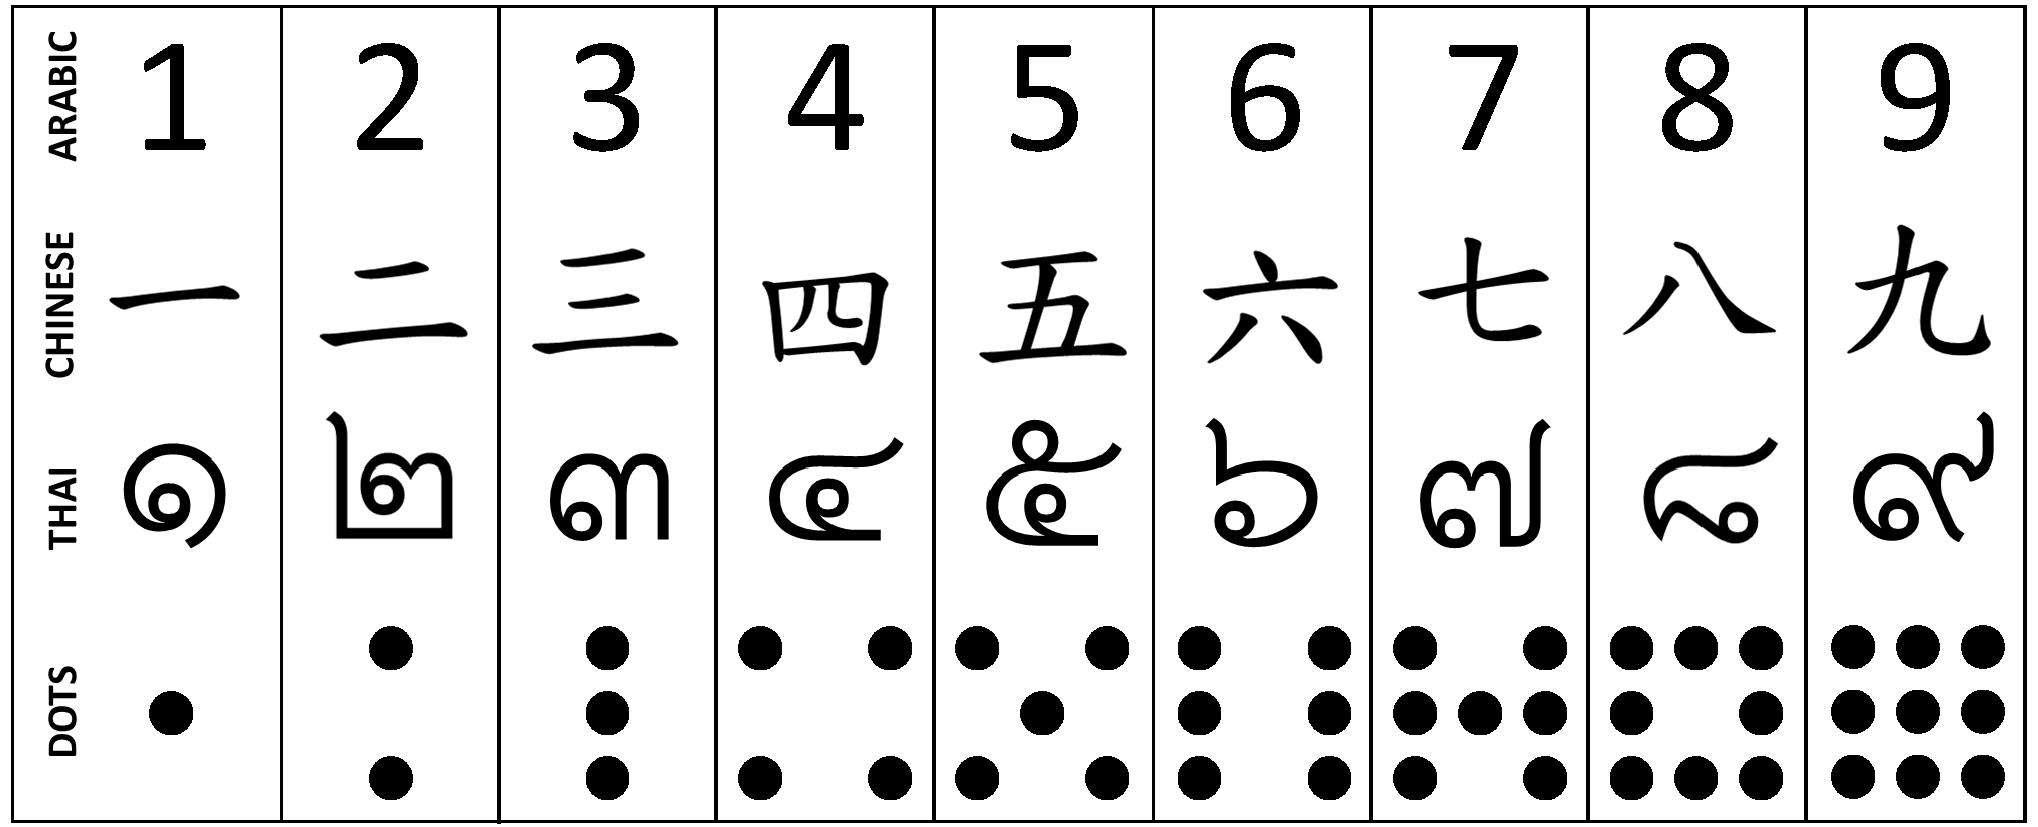
\includegraphics[width=\linewidth]{Figures/Wheel/NumStim.pdf}
\caption{Arabic, Chinese, Thai and dot numerals for the range of one to nine (left to right).}
\label{fig:Wheel_NumStim}
\end{figure}

Target stimuli were displayed in the center of the screen within a noisy field \cite<$\mu$ = 0, $\sigma$ = 0.125; à la>{eidels2014measuring} and were followed by a central backwards-mask. At a viewing distance of 60cm, each noisy target stimuli subtended a visual angle of 5.53 degrees (5.8cm$^2$) and the mask subtended a visual angle of 11.61 degrees (12.2cm$^2$). Responses were made by moving the mouse to the matching numeral presented within a response-wheel (see Figure \ref{fig:Wheel_SlideOrder}). The response-wheel was evenly divided into nine sectors, each containing one of nine numeric-symbols. The symbols were sampled from one of the four numeric-conditions (Arabic, Chinese, Thai and Dots; see Figure \ref{fig:Wheel_NumStim} again). Each numeral was randomly allocated to a wheel sector at the start of each session and displayed equidistant from the starting mouse location. This design ensured no one numeral was spatially biased towards the target.

At the start of each response-window, a mouse-cursor appeared in the center of the number-wheel. Participants responded by moving the mouse-cursor towards the segment that contained the best match to the previously presented stimulus. A response was taken once the cursor passed over the inner-circle of the response-wheel. At a viewing distance of 60cm, the inner-circle of the response-wheel subtended 20.04 degrees visual angle (diameter 21.2cm) and the outer-circle subtended 25.91 degrees visual angle (diameter 27.6cm). All experimental displays were presented on a gray background with RGB values (240, 240, 240). 

\subsection{Procedure}
Participants completed four 90min sessions --- Arabic, Chinese, Thai and non-symbolic dots. Session order was randomized using a Latin-square design. At the start of the first session participants were presented an information statement and provided signed consent before answering demographic questions regarding age, gender, handedness and vision. Participants reported whether they identified as being proficient in English, Chinese and Thai. At the start of each session participants were instructed to briefly view a noisy symbol, and using the mouse, identify the best matching symbol on the response-wheel.

Each trial began with a blank screen presented for 250ms, followed by a central fixation-cross for 500ms, followed by a 250ms blank screen. The stimulus display was then presented for 500ms, followed by a mask for 200ms. The response-window began at the presentation of the response-wheel and lasted 8000ms (see Figure \ref{fig:Wheel_SlideOrder}). A trial ended when a response was made or when the trial timed-out. 

% Trial Order Slide
\begin{figure}[tbh]
\centering 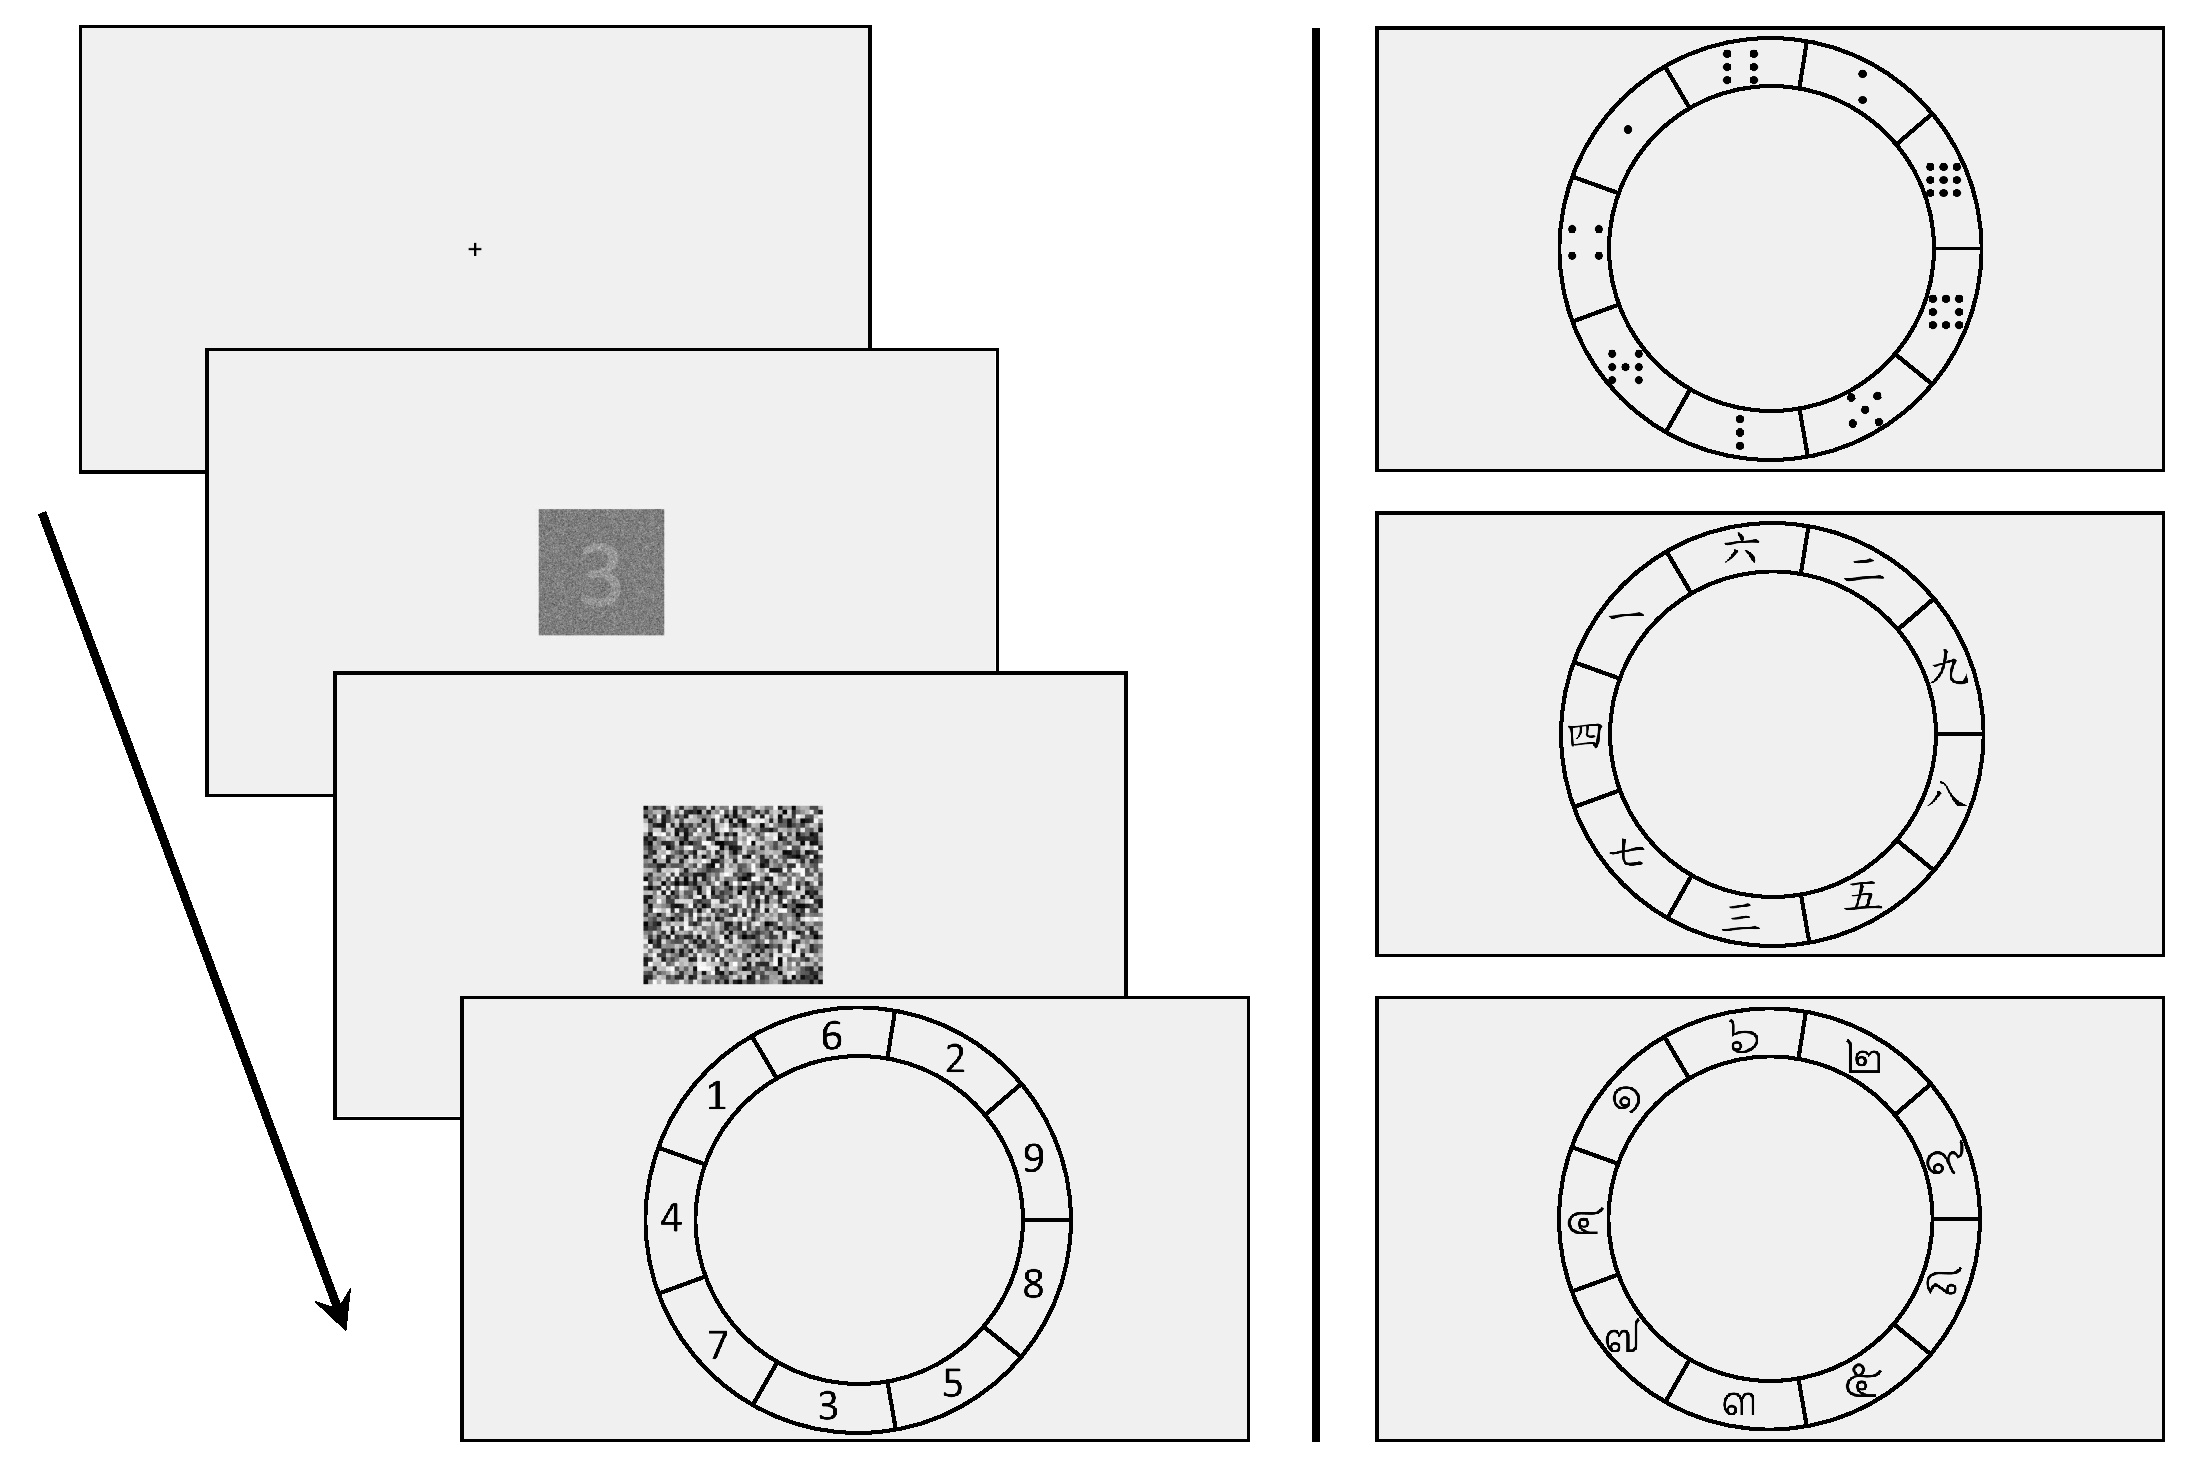
\includegraphics[scale = .37]{Figures/Wheel/TrialOrderSlide.pdf}
\caption{Illustration of a trial with Arabic numerals (left). Alternative response-wheels are displayed (right) for the non-symbolic dots (top), Chinese (middle) and Thai (bottom) numerals. For illustrative purposes, the position of each numeral is held constant between numeric-types.}
\label{fig:Wheel_SlideOrder}
\end{figure}

% Staircase Procedure
At the start of each session, participants completed a practice-calibration block. By means of a single staircase procedure, we manipulated the contrast of the signal across trials according to the participant's responses. A modified 2-up 1-down rule was applied\footnote{A classical 2-up 1-down staircase requires two correct responses on each step to step-up. Our modified staircase required a correct response on two contiguous trials, (\eg trial n-1 and trial-n), to step-up. This produced a faster and more responsive staircase procedure.}. Signal contrast began at a fixed RGB value (153, 153, 153), with two contiguous correct responses decreasing the RGB signal-values by 1 (becoming harder), and a single incorrect response increasing the RGB signal-values by 1 (becoming easier). This staircase design allowed participants to quickly plateau at their perceptual threshold. Earlier piloting with this procedure resulted in approximately 60\% accuracy in the main task. 

% Five Contrast Levels
Our proffered analysis technique, multidimensional scaling, requires a combination of correct and error responses. To ensure this, experimental stimuli were presented at five signal levels of varying difficulty \cite<following>{eidels2014measuring}. A critical contrast level was determined by the mean RGB values of the final 30 calibration trials. The highest signal level (easiest) was presented three RGB steps above the critical contrast. The lowest signal level (hardest) was presented one RGB step below the critical contrast. Together, these formed the five stimulus-signal contrast-levels. 

% Trials and Blocks
During each session, participants completed one practice block of 135 trials, and 13 experimental blocks each containing 90 trials. During an experimental block, each numeral was presented 10 times, twice at each of the five signal levels. Trial-by-trial accuracy feedback was provided during the practice-calibration block and trial order was randomized within each block. Block accuracy was displayed as a graph at the end of each experimental block to encourage participant engagement\footnote{At no point during the experiment were any numbers displayed except for those contained by the response-wheel and target-stimulus. Accuracy was presented as a line graph with no numbers, and countdown timer was displayed as a ticking sundial.}. In total, each participant completed 130 experimental trials per numeric-symbol, and 1170 experimental trials per-session. 

\subsection{Data Analysis}
Trials with no response were removed from the analysis. Calibration (practice) and experimental trials were assessed for accuracy to ensure an appropriately difficult stimulus-signal contrast was achieved. Repeated-measures ANOVAs and paired-sample \textit{t}-tests were used to statistically compare differences between numeric sets. Where accuracy was matched by signal-contrast level, between-subject ANOVAs and independent-samples \textit{t}-tests were used. Multiple comparisons were corrected for family-wise error using the bonferroni method.

For each participant, a 9 x 9 confusion matrix was generated for each numeric-type. To remove the effect of response-bias before MDS analysis, Luce's (1963) similarity choice model was applied to each confusion matrix. This model describes identification responses as probabilistic outcomes driven by the similarity of a stimulus to other in the choice set, as well as a response-bias parameter --- one for each stimulus. By estimating the parameters of the model, researchers can examine the theoretically meaningful similarity scores free from the effect of response-bias that can contaminate the observed data. In supplementary materials S4\ref{Appendix:Luce} we provide a formal description of Luce's choice model and describe the application to the current data. 

After application of Luce's choice model, non-metric multidimensional scaling was conducted on the bias-free similarity matrices. For each participant and each numeric-condition, a scree analysis was conducted to determine the appropriate number of MDS dimensions. Group MDS plots were generated for each numeric-type using the individual differences scaling (indscal) MDS technique \cite{carroll1970indscal}. Indscal provides a group MDS fit by deferentially weighting the contribution of each individual to the overall MDS fit. K-means cluster analysis was applied to determine cluster patterns at both the group level and across individuals. The frequency at which items clustered were turned into proportions and displayed as a heatmap, separately for each numeric-type. Finally, we compared MDS and K-mean cluster results to an ideal observer analysis, used to simulate pure perceptual confusions of the numeric sets.

\section{Results}
\subsection{Calibration Block}
Figure \ref{fig:Staircase} (top) depicts the calibration block for participant S1, responding to Arabic numerals. This staircase procedure was typical of all participants. The mean contrast level of the final 30 assessment trials (highlighted yellow) determined the critical contrast value --- the value from which stimulus-signal levels were determined in the experimental session. Violin plots (bottom) depict the mean and standard-error of contrast values for assessment trials, for each participant and numeric-type. Critical contrast levels were relatively stable across numeric-type and participants. 

% Staircase Figure
\begin{figure}[tbh]
\centering 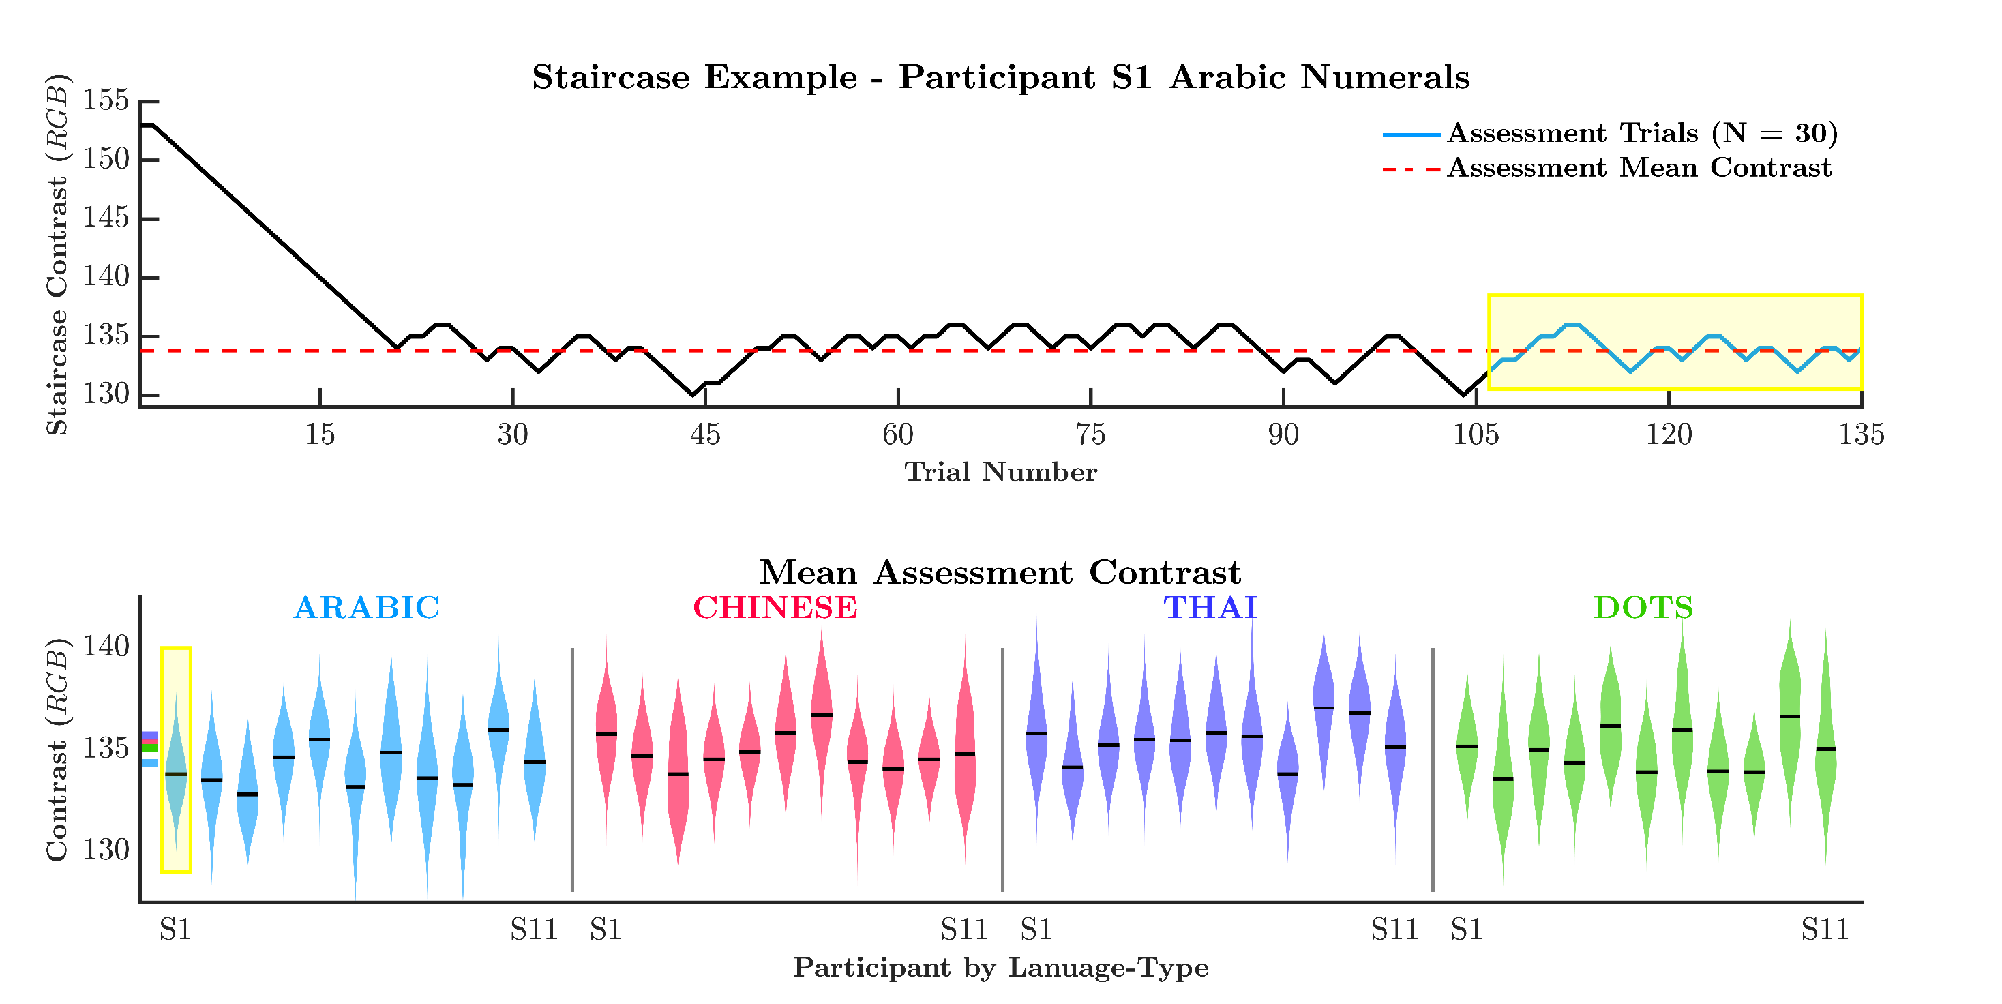
\includegraphics[width=\linewidth]{Figures/Wheel/Staircase.pdf}
\caption{Plot of participant S1's Arabic numeral staircase procedure (top) and violin plots of individual participant's staircase assessment trials (bottom). Assessment trials (highlighted yellow for participant S1) determined the critical contrast value for the main experiment. For all numeric-types, participants displayed relatively stable contrast levels during the assessment window. Black lines on each violin plot represents the critical contrast value (mean RGB value over the assessment window). Colored ticks on the y-axis are the mean critical contrast values for each numeric-type.}
\label{fig:Staircase}
\end{figure}

Colored ticks on the violin-plot (Figure \ref{fig:Staircase}, y-axis) show, on average, critical contrast levels were lowest for Arabic numerals (RGB $\mu$ = 134.14, $\sigma$ = 1.07), then non-symbolic dots (RGB $\mu$ = 134.88, $\sigma$ = 1.04), then Chinese numerals (RGB $\mu$ = 134.91, $\sigma$ = .86) and finally, Thai numerals (RGB $\mu$ = 135.5, $\sigma$ = .97). A lower signal-level suggests familiar numeric sets (Arabic and Dots) were easier to recognize than unfamiliar numeric sets (Chinese and Thai). However, the greatest difference between contrast levels, Arabic vs Thai, was only equivalent to a single RGB step.

\subsection{Experimental accuracy}
The staircase procedure was effective at reducing identification accuracy during experimental trials. On average, accuracy was highest for Chinese numerals ($\mu$ = .60, $\sigma$ = .21), then Arabic ($\mu$ = .59, $\sigma$ = .19) and non-symbolic dots ($\mu$ = .59, $\sigma$ = .19), and finally, Thai numerals ($\mu$ = .54, $\sigma$ = .19). Our manipulation of contrast accuracy was similarly effective. During experimental trials, stimuli were presented at five signal-levels, one step below the critical contrast value (level 1: hardest), at the critical value (level 2) and three steps above (levels 3, 4 and 5; easiest). As intended, mean accuracy increased linearly with the visibility of the contrast levels, being lowest at level 1 ($\mu$ = .32, $\sigma$ = .02) and highest at level 5 ($\mu$ = .80, $\sigma$ = .03). A full analysis of accuracy over contrast levels is provided in supplementary materials S4\ref{Appendix:contrastAcc}. For now, we  summarise by stating our manipulation of contrast worked as intended and produced error rates sufficient for our subsequent analyses.


\subsection{Response Bias}
Figure \ref{fig:AccRspFq}.a. shows the positive relationship (rank-order correlation $\rho$ = .83***) between response-frequency (blue) and response-accuracy (orange) for Arabic numerals in participant S1. Here, as the frequency of responding with a specific numeral, for example `4', increases, so too does identification accuracy. Similarly, as response-frequency decreases, such as with item `3', accuracy also decreases. This figure clearly displays the relationship between response-frequency (`strength' in Luce's choice model) and response-accuracy. 

The dotted blue line in Figure \ref{fig:AccRspFq}.a represents a response-frequency matching the number of stimulus presentations. For example, a `5' response was made as often as `5' was presented, however, these responses were correct only half of the time. By contrast, a `4' response was made nearly twice as often as it was presented, showing an effect of response-bias. The positive relationship between response-frequency and response-accuracy is evident when we examine the scatter plot in Figure \ref{fig:AccRspFq}.b. This scatter plot depicts accuracy against response-frequency (bias) for each participant, for each stimulus and numeric-type. The positive relationship ($r$ = .58***) indicates that in a standard analysis, overall accuracy and response bias could be mistakenly conflated. This highlights the need for a bias free measure of similarity, as offered by Luce's choice model.

\begin{figure}[tbh]
\centering \includegraphics[width = \linewidth]{Figures/Wheel/AccuracyResponseFreq.jpg}
\caption{a) Response frequency by response accuracy for participant S1, Arabic numerals. b) Scatter plot depicting a positive correlation between mean stimulus accuracy and response frequency, across numeric-types. c) Response frequency by response accuracy for stimuli for the Arabic (left), Chinese (mid-left), Thai (mid-right) and Dot (right) numeric-types.}
\label{fig:AccRspFq}
\end{figure}

Figure \ref{fig:AccRspFq}.c shows the mean response-frequency and mean response-accuracy of each stimulus, separately for each numeric-type. Averaging response-frequency and accuracy diminishes their correlation, however, clearly illustrates response patterns and accuracy for each stimulus. Together, these results show how an increase in response-frequency (or strength in Luce's choice model) can artificially improve identification accuracy for any given stimulus. Similarly, these results show how a decrease in response-frequency can lead to poorer stimulus identification accuracy. To understand the impact response-bias has on confusion data and our analysis of the mental space, we now consider our MDS results.

\subsection{Multidimensional Scaling}
\subsubsection{Response bias}
Figure \ref{fig:Bias2Unbias} shows MDS results from a representative data set (participant S4)  where response-bias was unaccounted for (biased plots) and corresponding MDS results where response-bias was removed from the data using Luce's choice model (bias-free plots). Changes between item-proximity within each numeric-type (blue arrows) illustrates how response-bias alters the MDS solution. All future references to MDS within the results section will pertain to the bias-free MDS solutions.

\begin{figure}[tbh]
\centering \includegraphics[scale = .48]{Figures/Wheel/BiasToUnbiasSingle.jpg}
\caption{Biased (uncorrected) and bias-free (Luce's choice model corrected) MDS solutions for participant S4, displayed separately for each numeric-type. Changes in item-proximity between biased and bias-free MDS plots displays the influence of response-bias on the MDS solution. \\\textbf{Note.} Numerals displayed within the MDS plots are for illustrative purposes and are not identical to the experimental stimuli; see Figure \ref{fig:Wheel_NumStim}. Dots are presented as Arabic numerals to avoid misinterpretation where numerals spatially overlap.}
\label{fig:Bias2Unbias}
\end{figure}

Scree analysis identified two-dimensions as an appropriate MDS representation for most participants in each of the four numeric-types (for more details see supplementary materials S4, Figure \ref{fig:Apx_ScreeEngDot} and Figure \ref{fig:Apx_ScreeChnThi}). Scree analysis identified three-dimensions as the appropriate MDS representation for three participants in the Arabic and Thai numeric-types, and the appropriate representation for four participants in the Chinese numeric-type. Individual bias-free MDS plots are displayed in supplementary materials S4, Figure \ref{fig:Apx_MDSenglish} -- Figure \ref{fig:Apx_MDSthai}; biased MDS plots are displayed in supplementary materials S4, Figure \ref{fig:Apx_MDSenglishBiased} -- Figure \ref{fig:Apx_MDSthaiBiased}). To describe trends observed across participants, we conducted an Individual Differences Scaling (indscal) MDS analysis. Results of the three-dimensional MDS indscal solutions (see supplementary material S4, Figure \ref{fig:Apx_3D_Indscal}) closely resemble the results of the two-dimensional MDS solutions. For efficiency of exposition, the following will focus on the majority of participants and the two-dimensional indscal results.

\subsubsection{MDS indscal interpretation}
Figure \ref{fig:Indscal} displays the group MDS indscal solutions for data collapsed across those participants best represented by two-dimensions, separately for each numeric-type. Interpretation of MDS plots is at times arbitrary and relies on visual inspection of the plots. Similarly, interpretation of the MDS solution's axes are also arbitrary with reference to the x- or y-axes \cite<see e.g.,>{nosofsky1986attention, nosofsky2018toward}. Likewise, the notion of similarity is very broad and has been the centre of many disputes in the literature \cite<e.g.,>{tversky1977features, medin1993respects}. We begin with a visually-guided assessment of the MDS plots, and then move to more formal analyses of clustering (using K-means cluster analysis) and similarity (using a rudimentary yet useful ideal-observer analysis). 

Arabic numerals appear to be arranged along dimensions of roundness (x-axis) and openness \cite<y-axis; similar results were observed by>{godwin2014numSim}. Arabic numerals formed four groups in the MDS space: [2,7], [1,4], [5,6] and [3,8,9]. The dimension of openness best described the diagonal of the y-axis\footnote{The rotation and direction of items within the MDS solution, relative to the x- and y-axis, is arbitrary. It is only important that these dimensions are orthogonal to one-another.} for all numerals except the closed shape of item `8'. Under noisy stimulus conditions, the concave exterior of `8' might be perceived as more `open' than it would under ideal viewing conditions. These results show an apparent effect of perceptual similarity on the mental representations of Arabic numerals.

\begin{figure}[tbh]
\centering 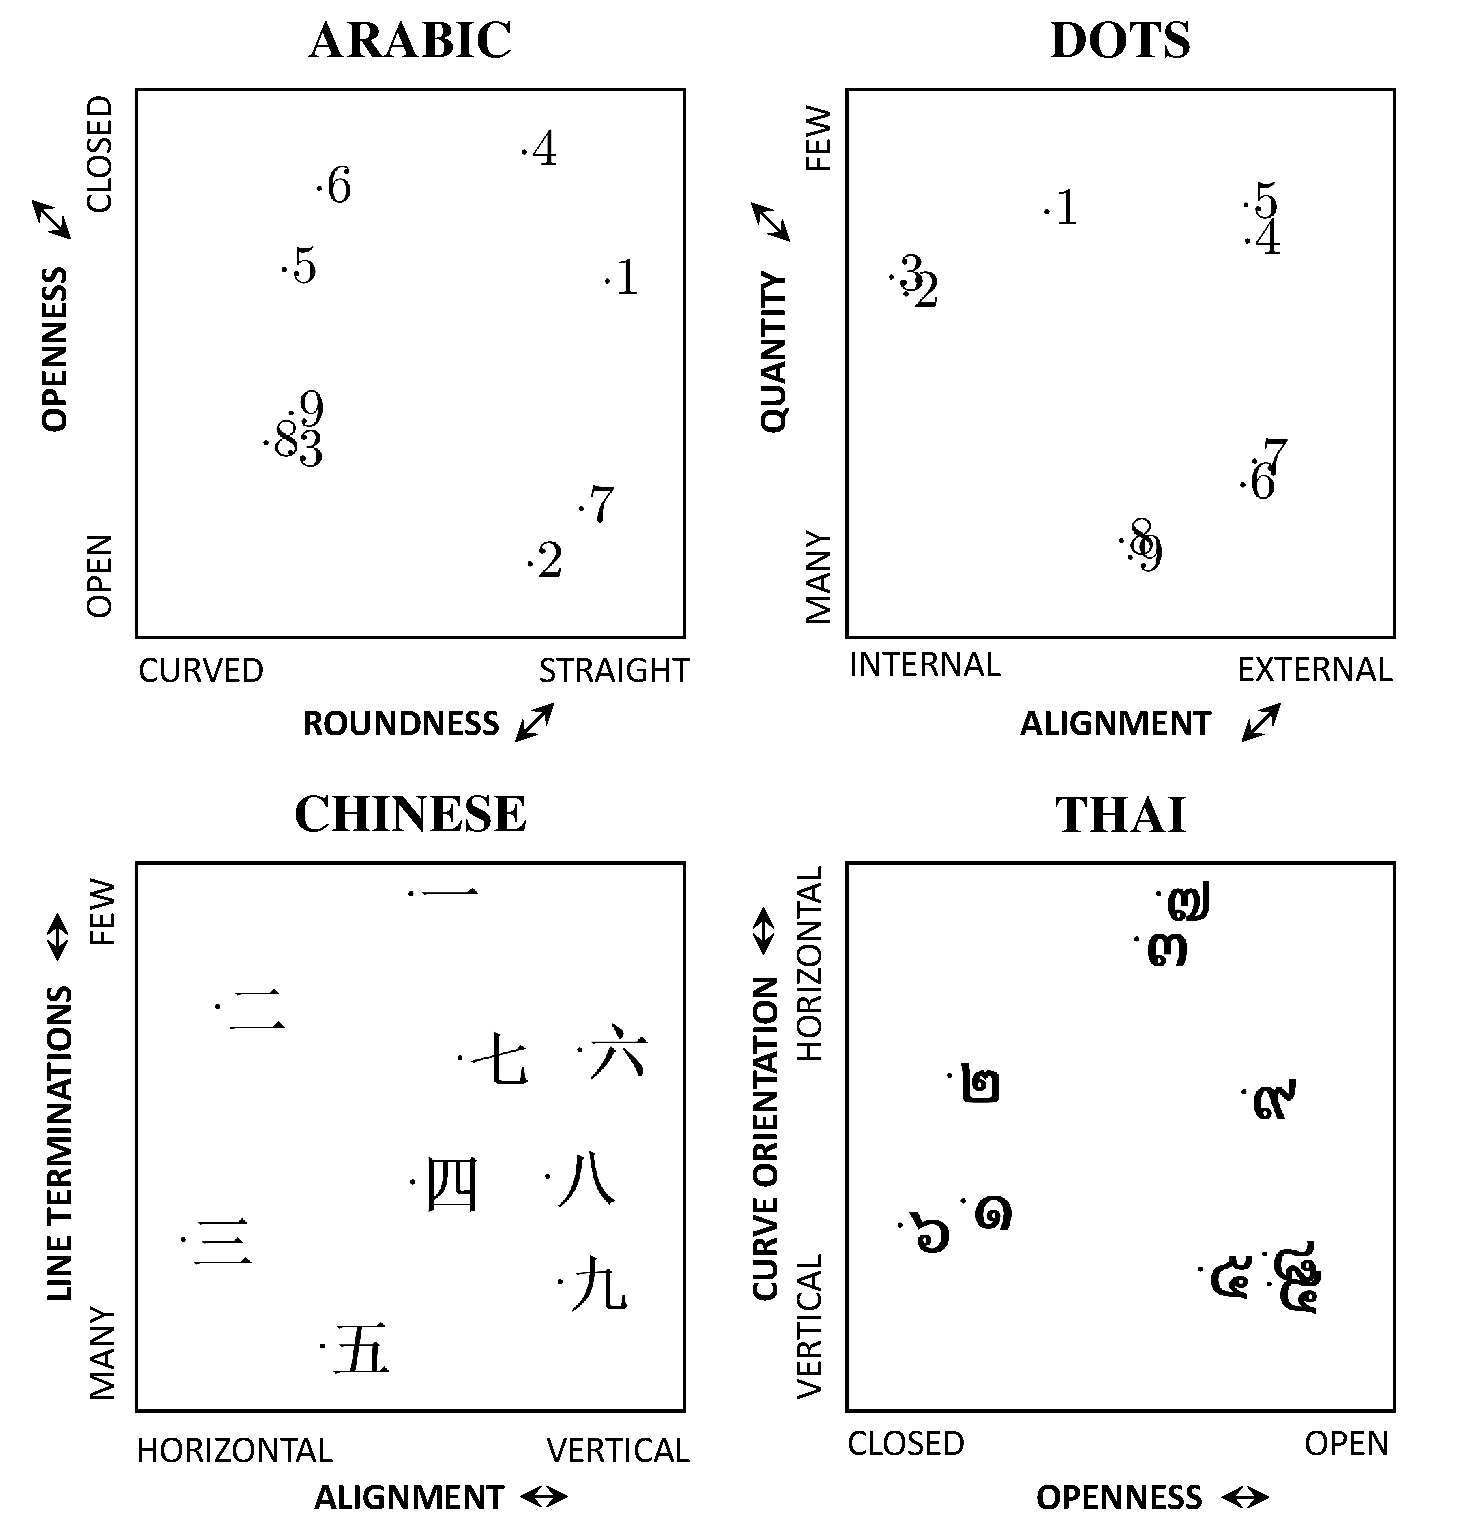
\includegraphics[scale = .45]{Figures/Wheel/IndscalDescription.pdf}
\caption{Individual differences scaling (indscal) solution for all participants best represented by a two-dimensional MDS space, displayed separately for each numeric-type. Dimensional labels and directionality (arrows) are displayed on the y-axis and x-axis.}
\label{fig:Indscal}
\end{figure}

The non-symbolic dots indscal MDS solution (Figure \ref{fig:Indscal}) appears to be displayed across dimensions of alignment (x-axis; whether items are presented internally or externally in the nine-dot array) and quantity (y-axis). Non-symbolic dots show five distinct groupings: [1], [2,3], [4,5], [6,7], [8,9]. These groupings suggest items cluster by numerical proximity. Furthermore, if we ignore the unique case of one-dot, numerical magnitude increases in a clock-wise direction, possibly reflecting the mental number-line. These results show an apparent effect of numerical magnitude and perceptual similarities on the mental representations of non-symbolic dots. 

The Chinese indscal MDS solution (Figure \ref{fig:Indscal}) appears to be arranged across dimensions of alignment (x-axis) and line terminations (y-axis). Chinese numerals are logographic, a trait captured by the visual property of alignment. As a consequence, small-magnitudes and large-magnitudes are mostly separate within the MDS space. Within this space, the Chinese numerals show three distinct groupings, \begin{CJK}{UTF8}{gbsn} [一, 二], [三, 五] and [四, 六, 七, 八, 九].\end{CJK} It is unclear whether the largest group might be better classified as two or three sub-groups, for example, \begin{CJK}{UTF8}{gbsn} [四], [六, 七] and [八, 九].\end{CJK} These results show an apparent effect of perceptual similarity on the mental representations of Chinese numerals.

The Thai indscal MDS solution (Figure \ref{fig:Indscal}) appears to be arranged across dimensions of openness (x-axis) and curve orientation (y-axis; \ie whether item curvature is horizontally or vertically aligned). Thai numerals show four distinct groupings: numerals with a vertical curve (numerals [3, 7]), numerals with a horizontal curve (numerals [4, 5, 8]), numerals with a closed shape (numerals [1, 2, 6]), and the solo group of item nine. These results show a clear effect of perceptual similarity on the mental representations of Thai numerals. 

Based on visual inspection, indscal MDS solutions provided an accurate representation of individual participant MDS results. Arabic, Chinese and Thai numerals were represented within the mental space across dimensions of perceptual similarity. Non-symbolic dots were represented within the mental space using dimensions of numerical and perceptual similarity. Indscal analysis is useful for identifying latent MDS dimensions, however, does not provide a formal measure of item-clustering. 

Deciding which items group together and which items are independent is a difficult process. For example, visual inspection of the Arabic indscal solution suggests items `1' and `4' may cluster together or may be independent. Similarly, Chinese numerals \begin{CJK}{UTF8}{gbsn}[四, 六, 七, 八, 九]\end{CJK} may form one group, or three. The `strength' with which two numerals cluster, may determine the likelihood of their confusion within the mental space. To characterize the strength of item-clusters in each individual, and across two- and three-dimensional MDS solutions, we applied to the data a variant of K-means clustering analysis. 

\subsection{MDS clustering}
K-means is an iterative clustering technique used to identify item groupings within dense data sets. A number of randomly located centroids (K) are updated iteratively until the data set can be partitioned into `K' non-overlapping clusters. This method works well for large, dense data sets, however, experiences a notable limitation with small data-sets.

Identifying the correct number of centroids is difficult for small data sets. Two, three or four centroids may be adequate for a sample of nine items. However, cluster selection methods developed for large data sets will generally favor higher centroid counts, (\eg five or six centroids), at a risk to over-fitting the data. 

To overcome this limitation, we ran K-mean cluster algorithms using 2--6 centroids, on each bias-free MDS solution. On each iteration of `K', we recorded which items clustered together (Figure \ref{fig:Kmean}.a) to produced a measure of cluster frequency (Figure \ref{fig:Kmean}.b). For illustration, in the data presented in Figure \ref{fig:Kmean}.b, the digits '1' and '2' were clustered together three times (across the the fine clustering scenarios, K=2, K=3, ... K=6, illustrated in Figure \ref{fig:Kmean}.a), whereas the digits '1' and '4' were clustered together only one time. Of course, each digit is always clustered with itself, resulting in the maximum value of five along the main diagonal.

Within each numeric-type, cluster frequencies were summed across participants and represented by proportion (see Figure \ref{fig:HeatMapSubjects}.a). Separate heatmaps were calculated for two-dimensional and three-dimensional participants (supplementary material S4, Figure \ref{fig:Apx_2D_MDScounts} -- Figure \ref{fig:Apx_3D_MDScounts}). Being comparable, these results were collapsed into Figure \ref{fig:HeatMapSubjects}.a. This method was robust to the number of MDS dimensions, as clusters could be calculated in either two- or three-dimensional space. For direct comparison to the previously presented group indscal results, a separate cluster heatmap was generated using the two-dimensional indscal results (Figure \ref{fig:HeatMapSubjects}.b).

% Kmean Cluster Explainer
\begin{figure}[tbh]
\centering \includegraphics[scale = .45]{Figures/Wheel/ClusterExplainer.jpg}
\caption{a) K-mean cluster solutions for 2--6 clusters, for a single participant. K-mean cluster centers (centroids) are illustrated by `x' markers, and groupings are denoted by color. b) Cluster frequency heatmap for the same data. Darker colors indicate items which most frequently cluster together.}
\label{fig:Kmean}
\end{figure}

% Participant Response - Item Clusters
\begin{figure}[tbh]
\centering 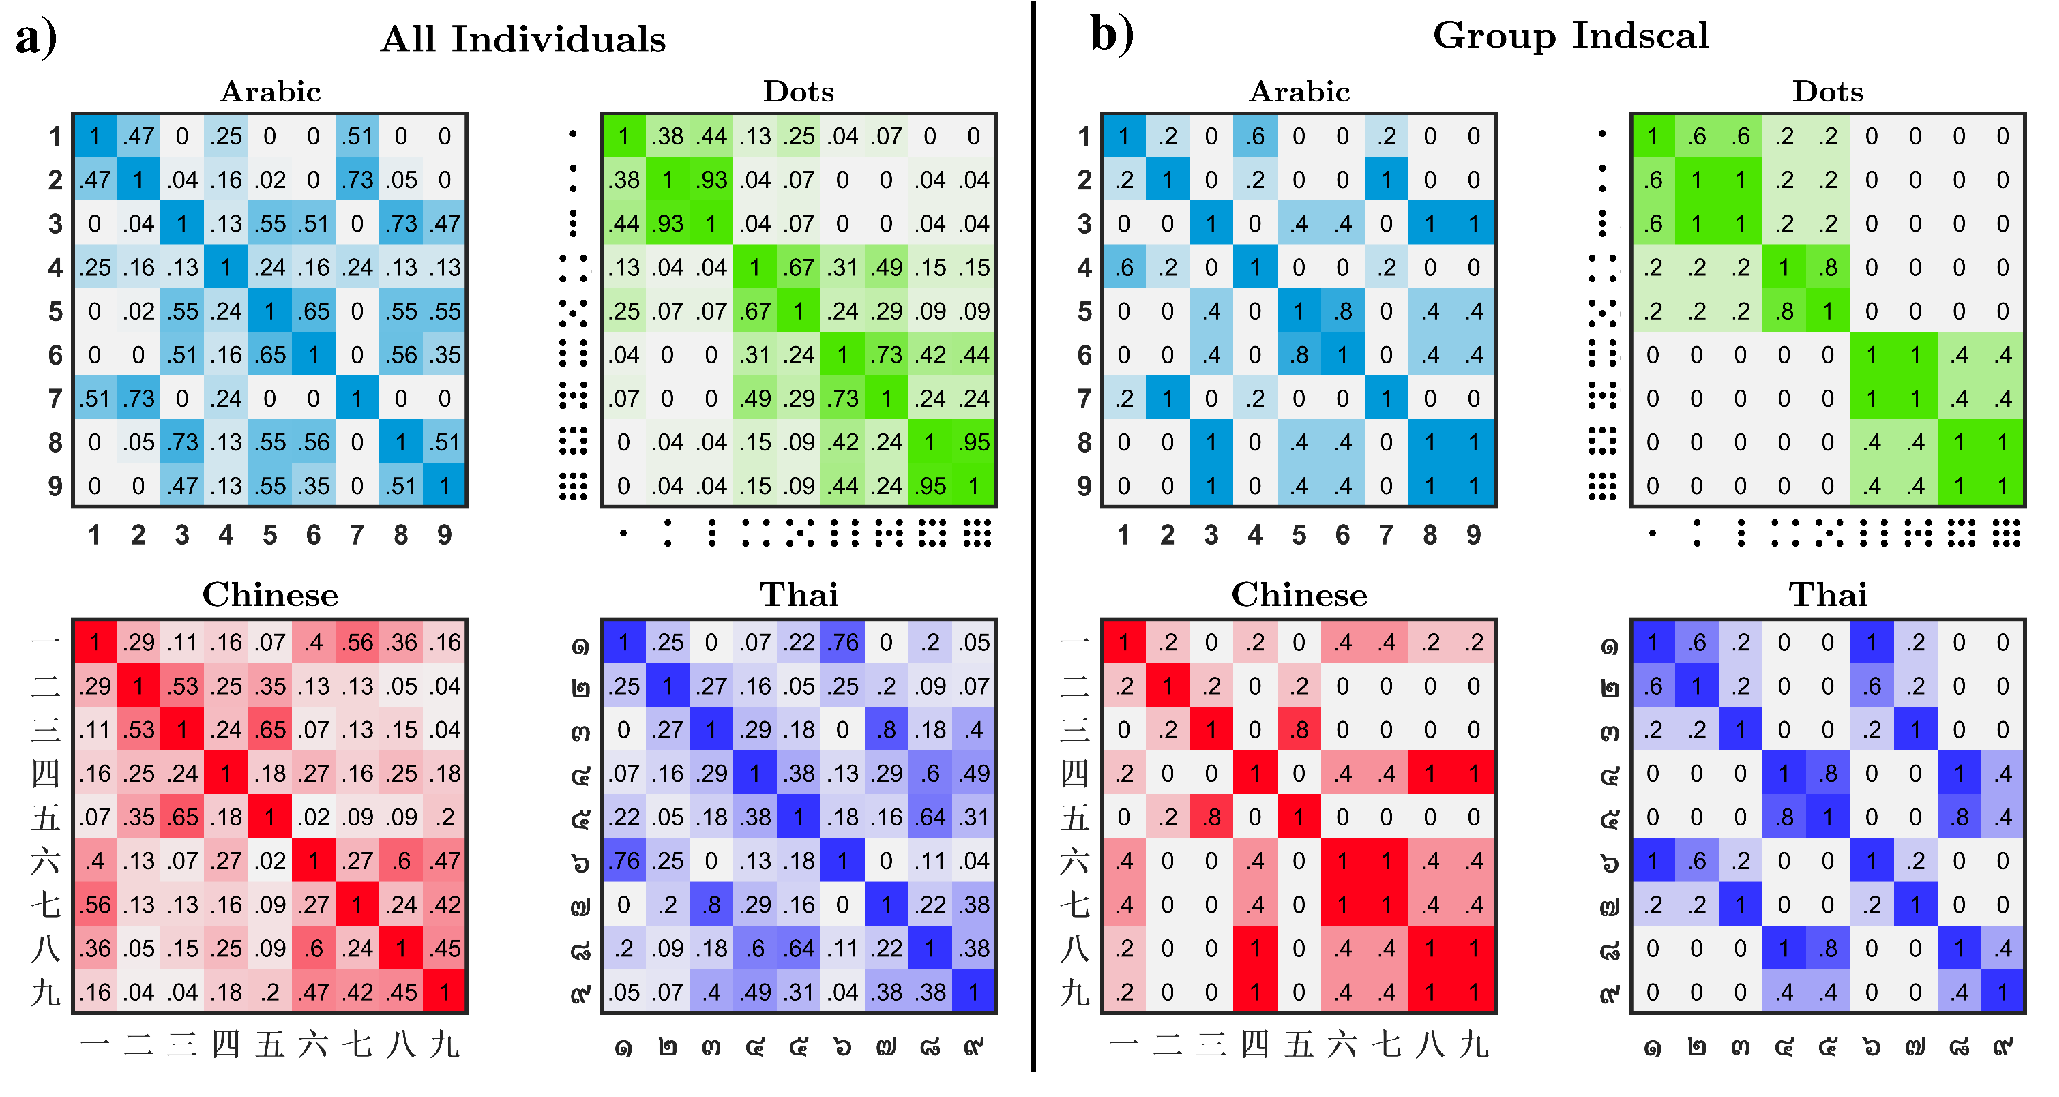
\includegraphics[width=\linewidth]{Figures/Wheel/IndivVsIndscalHeatmap.pdf}
\caption{a) Proportional cluster-frequency heatmap for all eleven participants (including both two- and three-dimensional MDS solutions), across 2--6 K-mean clusters. b) Group indscal two-dimensional MDS (Figure \ref{fig:Indscal}) cluster-frequency heatmap, across 2--6 K-mean clusters. Larger proportions (darker colored squares) indicate items which most frequently cluster together.}
\label{fig:HeatMapSubjects}
\end{figure}

% Arabic Clusters
The top-left of Figure \ref{fig:HeatMapSubjects}.a displays the proportion by which items clustered across individuals, for Arabic numerals. Across individuals, the strength of items clusters generally aligned with the group indscal results (top-left, Figure \ref{fig:HeatMapSubjects}.b). In line with the indscal MDS solution, items with similar perceptual properties, for example, the items [3, 5, 6, 8, 9] share the perceptual property of `roundness', while [2, 3] share the property of `openness'; frequently clustered across individuals. Cluster patterns displayed no effect of numerical proximity (neighbouring items clustered infrequently). These results support the indscal analysis, and suggest that at the individual level, Arabic numerals were clustered strongly by the perceptual properties of `curvature' and `openness'. 

% Dot Clusters
The top-right panel of Figure \ref{fig:HeatMapSubjects}.a displays the proportion of item-clustering for non-symbolic dots. The left-to-right diagonal pattern of results, radiating outwards towards zero in the opposite corners, suggests items clustered by numerical proximity. Yet, items close in numerical proximity cluster together in staggered item-sets. For example, items [2, 3], [4, 5] and [6, 7] cluster, but rarely [3,4], [5,6] or [7,8]. This pattern of results is made clearer by the group indscal plot (Figure \ref{fig:HeatMapSubjects}.b). This staggered pattern of results is not accounted for by numerical proximity, but rather, perceptual similarities. 

% Staggered Dot Clusters
Staggered clusters, such as 4 and 5 dots, share similar perceptual characteristics, and differ only by the location of a single, central dot. Mental distance between dot representations are likely confounded by both perceptual similarity and numerical proximity; minimal changes such as adding one dot result in minimal changes to both quantity and visual appearance, and likewise adding a large number of dots to a display results in substantial changes to both quantity and visual appearance. As such, it could be that our observed clusters are due to i) only perceptual, ii) perceptual \textit{and} numerical, or iii) only numerical similarities. Results from the indscal MDS solution suggested items were confused along dimensions of quantity (numerical) and alignment (perceptual). As such, it seems likely this staggered pattern reflects a combination of numerical and perceptual similarities.

% Chinese Clusters
The bottom-left panel of Figure \ref{fig:HeatMapSubjects}.a displays cluster frequencies for Chinese numerals across individual participants. These results do not align with numerical-proximity, (\eg non-symbolic dots heatmap), and suggests items clustered by perceptual similarity. Noisy, low-frequency item-clusters are common for Chinese numerals, reflecting the unfamiliar nature of this numeric set with our cohort. Moderate cluster frequencies are present between numerals \begin{CJK}{UTF8}{gbsn} [二, 三, 四, 五] and [六, 七, 八, 九]\end{CJK}. The items within these groups are --- unbeknownst to our participants --- numerically contiguous. This clustering might reflect the logographic nature of the Chinese numeric-set and the perceptual similarities within smaller and larger magnitudes. 

% Chinese clusters - perceptual
With increases in magnitude, Chinese numerals shift from horizontal to vertical alignment, creating perceptual similarities within smaller and larger magnitudes. Furthermore, smaller magnitudes are generally represented by fewer line-features, (\ie line-endings), than larger magnitudes. Subsequently, perceptual similarities are strongest within smaller and larger magnitudes. This accounts for the observed indscal MDS results (Figure \ref{fig:HeatMapSubjects}.b) and cluster frequency results. Together, these analyses suggest that at the individual level, Chinese numerals are strongly influenced by the perceptual properties of `alignment' and `line-endings'. 

% Thai Clusters
The bottom-right panel of Figure \ref{fig:HeatMapSubjects}.a displays cluster frequencies for Thai numerals. Similar to Chinese numerals, Thai cluster patterns do not align with numerical proximity and display an abundance of low-frequency clusters. This may reflect the unfamiliar nature of the numeric-set. Across individuals, and at the group level (Figure \ref{fig:HeatMapSubjects}.b), high cluster frequencies are apparent between item numbers [1,6], [3,7], [4,8], [4,5] and [5,8]. Notably, these items share perceptual features of `roundness' and `curvature orientation'. Supplementing these findings with the previous indscal MDS analysis, results suggest that at the individual level, Thai numerals clustered strongly by the perceptual properties of `curvature orientation' and `roundness'. 

% Summary of Cluster Results
Supplementing indscal analysis with cluster frequency heatmaps, our results indicate perceptual similarity strongly influenced the confusion of Arabic, Chinese and Thai numerals. Furthermore, perceptual similarity also influenced the confusion of non-symbolic dots, but could be confounded with numerical distance in this set, as explained above. Determining the fidelity of these claims is difficult without a benchmark model for comparison. To this end, we now present simulated results from a simple ideal observer analysis. 

\subsection{Ideal Observer Analysis}
% IOA Method
The ideal observer analysis is a simple template matching process that compares numeric stimuli, pixel-by-pixel, to generate a confusion matrix. The ideal observer is $not$ a model of human performance, but rather, a benchmark against which we may compare the performance of human observers \cite<\eg>{gold1999identification, eidels2014measuring}. The `ideal observer' compares a noisy numeric stimulus to all possible templates, for example comparing a noisy `1' stimulus to the numerals `1--9'. The template with the best cross-correlational match over many iterations, with randomly sampled noise, is selected as the `ideal observer response'. Normally distributed noise ($\mu$ = 0, $\sigma$ = [1.065, .12, 1.127, 1.463] for Arabic, dot, Chinese and Thai numerals, respectively) is added to each numeric stimulus, until the ideal observer's accuracy resembles the average accuracy of the participants. This process was repeated 10,000 times, per numeric-stimulus, per numeric-type, generating four confusion matrices. 

% IOA Figures
To afford a direct comparison to the collected participant data, Luce's choice model was applied to the simulated ideal observer data. Figure \ref{fig:IOA}.a displays the bias-free MDS solutions generated by the ideal observer. Figure \ref{fig:IOA}.b displays the corresponding K-mean cluster frequency heatmaps. These Figures provide a benchmark of performance, given numeric-stimuli were only confused by perceptual similarities.

% Figure: IOA MDS and Heatmap 
\begin{figure}[tbh]
\centering \includegraphics[scale = .4]{Figures/Wheel/IOA2.jpg}
\caption{a) Ideal observer analysis bias-free MDS solutions, generated separately for each numeric-type. Non-symbolic dots are displayed as Arabic numerals in the MDS plot for clarity to the reader. b) Ideal observer K-mean cluster frequency heatmaps.}
\label{fig:IOA}
\end{figure}

% IOA vs Arabic
Comparing Arabic indscal MDS results (Figure \ref{fig:Indscal}.a) to the Arabic ideal observer MDS results (Figure \ref{fig:IOA}.a), we observe differences between item proximities and co-occurring item groups [2, 7] and [5, 6]. Comparing cluster frequency heatmaps, we find co-occurring item-clusters [1, 2], [2, 7], [5, 6], [5, 9] and [6, 9], suggesting participants confused these items due to perceptual similarities. Other item-clusters did not co-occur even though Arabic numerals appeared to be confused along dimensions of perceptual similarity.

% IOA vs Dots
Indscal MDS results for non-symbolic dots differed greatly from the ideal observer, and only shared item groups [1, 5] and [6, 7]. Cluster frequency heatmaps were comparable for items [1, 3], [6, 7] and [6, 8], yet the remaining item clusters were markedly different. Participants appeared to represent non-symbolic dots along dimensions of perceptual \textit{and} numerical similarity. The differences between participant and ideal observer MDS and cluster frequency results may reflect the impact of numerical proximity on the mental space. 

% IOA vs Chinese
The Chinese indscal MDS solution shared similarities with the ideal observer MDS solution. Chinese numerals \begin{CJK}{UTF8}{gbsn} [一, 二, 七], [三, 五], [四, 九] \end{CJK} group in both participant and ideal observer MDS solutions. Cluster frequency heatmaps were similar for items \begin{CJK}{UTF8}{gbsn} [一, 六], [二, 三], [四, 九], [四, 六], [四, 六] and [六, 七] \end{CJK}; these items all share distinct horizontal line features. While many item clusters were observed in both participant and ideal observer results, the pattern consistent with a logographic numeric-set was not observed by the ideal observer. As with our comparison of Arabic numeral results, it appears the ideal observer is only sensitive to a limited set of perceptual similarities.

% IOA vs Thai
The Thai indscal MDS solutions shared similarities with the ideal observer MDS solution. Two MDS groups are distinctly apparent in both solutions, items with a vertical curve (item numbers 4 and 5) and items with a horizontal curve (item numbers 2, 3 and 7). These groups are reflected in the cluster frequency heatmaps (Figure \ref{fig:IOA}). The ideal observer analysis shows very little noise in item-clustering, suggesting that item clusters were determined by highly salient (and comparable) perceptual features. 

\section{Discussion}
% General Summary of Results
In the current study, participants were asked to identify a noisy symbol (numeral) using a stimulus response wheel. A staircase procedure ensured identification accuracy was approximately 60\% for all participants, regardless of numeric-type. Stimulus accuracy positively correlated with response-frequency, across all participants and numeric-types. The application of Luce's choice model negated the effect of response-bias from the multidimensional scaling solutions. MDS and cluster frequency analyses were used to determine the dimensions upon which items were represented in the mental space. Arabic, Chinese and Thai numerals were represented by dimensions of perceptual similarity, and non-symbolic dots were represented by dimensions of numerical proximity and perceptual similarity. MDS and cluster patterns generated by an ideal observer were similar for Chinese and Thai numerals, although, differed greatly for Arabic and non-symbolic dot numerals.

\subsection{Response Bias}
Response-bias had a significant effect on identification accuracy and the multidimensional scaling solutions. Luce's choice model removed response-bias from individual MDS solutions. This altered relative item-proximities and created more even-weightings between items. Indscal analysis collapsed results across bias-free MDS solutions, and allowed the interpretation of bias-free similarity dimensions within the mental space. To the best of our knowledge, this study provides the first ever bias-free representation of the mental space, for familiar and unfamiliar numeric-sets.

\subsection{Multidimensional Scaling}
The majority of participants in Arabic, Chinese and Thai numeric-types, and all participants in the non-symbolic dot numeric-type, were best characterised by two-dimensional MDS solutions. Where participants displayed a third MDS dimension, MDS and K-mean cluster frequency results were comparable, and no category label could be easily applied to the third similarity dimension. As such, the following will focus on the two dimensional MDS results.

\subsubsection{Arabic symbols}
In line with past findings \cite{godwin2014numSim}, Arabic numerals appeared to be arranged in MDS space by the perceptual dimensions of `roundness' and `openness'. Against predictions, familiarity with the Arabic numerals did not produce numeric-confusions. Participant MDS and K-mean cluster frequency heatmaps displayed limited similarities with the ideal observer analysis.

Items [1, 2], [2, 7], [5, 6], [5, 9] and [6, 9] were similarly represented by both participants and the ideal-observer. Item `6’ and `9’ are identical once rotated, and `5’, `6' and `9' share features of curvature. Items `2’ and `7’ share similar diagonal midsections, and a horizontal feature. These similarities relate to the `roundness' of the items and not the openness of their form. 

The ideal observer analysis was not sensitive to similarities of `openness’. Openness relates to the concave `absence’ within an item, and not an extant feature, for example, a straight-line. As openness may be poorly captured by a pixel-by-pixel comparison of similarity, many Arabic numerals that clustered in the participant data were not clustered in the ideal observer analysis.

% PG Updated with Distance Effect
\subsubsection{Non-symbolic Dots}
All participants displayed two-dimensional MDS solutions for non-symbolic dots and appeared to be arranged along dimensions of `quantity’ and `alignment’. MDS plots displayed a rotational ordering, with items progressing from smaller-to-larger magnitudes --- a possible representation of the mental number-line. Items [2, 3], [4, 5], [6, 7] and [8, 9] reliably clustered together. This might reflect numerical proximity and the numerical distance effect operating within the mental space. However, the staggered item-clusters may also be caused by perceptual similarities. Sadly, perceptual similarity and numerical distance are confounded in dot stimuli; adding (or subtracting) one dot from a given display results in a relatively small change to both numerosity and visual appearance, and likewise adding many dots changes substantially both numerosity and visual appearance. Future studies could potentially disentangle this confound, perhaps by orthogonally manipulating the size and quantity of the dots, to eliminate or at least minimize their co-variation. 

Staggered cluster-sets only differed by the presence/absence of a single central item and MDS patterns displayed an effect of dot alignment. This suggests an effect of perceptual similarity. A simple template-matching ideal observer did not produce the staggered cluster pattern displayed by participants. A model as simple as the one we applied is only sensitive to low-level visual similarity driven by spatial overlap, and has no knowledge of numerosity. However, because numerosity and perceptual similarity co-vary in the dot set we have tested, it is not possible to separate effects of numerical and perceptual distances on the mental representations of these stimuli. Future work could focus on manipulations that minimize the co-variation. 

The MDS dimension of alignment could be unique to the current dot stimuli. For example, this dimension may disappear if items were arranged in a circular pattern or in a different canonical form (e.g., dice patterns). Similarly, it is unclear whether the dimension of quantity would be displayed if dots were presented in randomised locations. Assessing how different canonical forms and randomised dot patterns affect the MDS space is another clear direction of future research.

\subsubsection{Chinese symbols}
In line with our predictions, Chinese MDS dimensions appeared to be arranged by perceptual dimensions of `line terminations’ \cite<as similarly found in letters,>{fiset2008features} and `alignment’ (horizontal vs vertical). K-mean cluster frequency patterns depict large cluster groups between item-numbers 2--5 and 6--9. This reflects the logographic nature of the numeric-set, an effect captured by the shift from horizontal ($<$ 5) and vertical ($>$ 5) alignment. Although the ideal observer replicated many Chinese numeral cluster patterns, the logographic cluster pattern was not. Instead, the ideal observer focused upon similarities in horizontal line features. 

Although Chinese numerals were unfamiliar to the tested cohort, the numeric-set displayed intuitive similarities between items of similar magnitude. This logographic feature may be useful numeric property. For example, an intuitive relationship between symbol and magnitude might help when initially learning the numeral system \cite{hung1992automatic}. Additionally, logographic numerals might aid the precision of numeric-communication within a Chinese speaking cohort, (\eg mistaking \begin{CJK}{UTF8}{gbsn}二 for 三\end{CJK} is less costly than mistaking 6 for 9).

\subsubsection{Thai symbols}
In line with our predictions, Thai MDS solutions were arranged by perceptual dimensions of `curve orientation' and `openness' \cite<as found in Arabic numerals,>{godwin2014numSim}. K-mean cluster frequency patterns depict many low-frequency clusters, suggesting uncertainty in participant responses. Yet, regular cluster-patterns were displayed between items sharing similar perceptual features --- a finding echoed by the ideal observer analysis. As predicted, Thai numerals did not display a logographic cluster pattern. Together, these findings show a clear effect of perceptual similarity on the mental space for the unfamiliar Thai numeric set. 

\subsection{Future research}
The current study tested an English speaking cohort, comparing multidimensional scaling solutions for familiar (Arabic and symbolic-dots) and unfamiliar (Chinese and Thai) numeric-sets. In the next Chapter, we will test this experimental design within a Chinese speaking cohort. We will then compare and contrast differences in these two cohort's mental representations. %This will not only provide insight into how the mental space changes across cultures, but also in response to differing levels of expertise. 

Arabic and Chinese symbols are common within Chinese speaking countries. As such, the mental representation of Arabic digits may be similar between cohorts, while Chinese symbols may be represented differently \cite<e.g.,>{yeh2003role}. These differences might reflect familiarity with the numeric-set, (\ie expertise), and an effect of numerical similarity. We would expect Thai symbols and symbolic dots to be represented similarly by both cohorts. However, with such different backgrounds, experiences and languages, these predictions are far from a forgone conclusion.

To disentangle perceptual from semantic effects in the mental space, we also propose two additional experiments: a perceptual matching task, and a semantic matching task. Following a similar spatial arrangement method to \citeA{godwin2014numSim} and \citeA{goldstone1994efficient}, we may ask participants to arrange the four numeric-sets into clusters that represent their i) perceptual similarities, and ii) semantic similarities. This method may i) further validate the perceptual results we observe in this task, and ii) examine the effect of semantic similarity on the mental space. Unfortunately, this study is beyond the scope of the current thesis. As such, we leave this task to future researchers. 


\subsection{Conclusions}
People often confuse the identity of numeric symbols. These confusions may be of little consequence, (\eg confusing `\$6' vs `\$9'), or a major inconvenience, (\eg confusing `2' vs `7' eggs in a cake mix!). Past research has examined the mental dimensions of numeric item-sets, however, these results were always confounded by participant response-bias. We have presented the first bias-free mental representations of familiar (Arabic and dots) and unfamiliar (Chinese and Thai) numeric-sets. We also compared symbolic and non-symbolic mental representations of quantity. Our findings show Arabic, Thai and Chinese symbols are represented by dimensions of perceptual similarity within the mental space. Representation of non-symbolic dots could be affected by either perceptual similarity or numerical proximity, or both, however, co-variation precludes a clear inference. A clear path forward from the current study is to replicate this work in Chinese or Thai speaking cohort. 

From mathematics to recipes, speed-signs to phone-numbers, our ability to perceive and communicate symbolic-quantities is critical to daily life. Understanding why fundamental cognitive mechanisms fail and confuse symbolic quantities is an important topic of human cognition. Aside from extending our understanding of numerical cognition, the findings of this study have applications in the development of future numeric fonts and item-sets. Such work must consider i) the perceptual dimensions upon which items differ, ii) whether items should convey implicit value, (\ie be logographic), and iii) how these factors may improve the rate of symbolic learning and minimize numeric confusions.

%%AE DONE 31/10/2019
%% i focused on the new changes in red, just remember to be careful with >>> the use of 'similarity' and your inference about perceptual vs numerical effects, and the interpretation of the MDS dimensions 